\section{Object Identification}
Given the gaze directions, in order to know which object is being looked at, we need to know the objects' locations.  For the purpose of the pilot study, we assumed object locations are fixed during the trial and calibrate their positions before the trial.


The calibration should be performed by a person whose 3D head model has been learned and whose eyes are part of the ALR training examples for best gaze estimation accuracy.  The person is asked to look at each object when prompted while walking around, and gaze directions are estimated then recorded.  The intersection of two gaze directions pinpoints an object's location.  However, because the objects are larger than pinpoints, and gaze direction predictions have errors, thus we describe each object location as a Gaussian ellipsoid, with mean and variance calculated from all recorded gaze directions.  The resulting Gaussian ellipsoid is shown in Figure \ref{fig:locCalibResults}.  The center of the Gaussian, shown in red, is calculated by finding the point in space closest to all gaze lines, shown in blue.  For the \(i^{th}\) gaze line given by \(P_{oi} + s_i U_i\) (\(s_i\) a scalar, \(P_{oi}\) a 3D vector, and \(U_i\) a 3D unit vector), and for P the 3D point denoting the center to be calculated, then setting \(s_i = (P - P_{oi})\cdot{U_i} \) gives the closest point on the line to P (shown as green dots).  Our problem can be formulated as finding a P that minimizes the sum of squared distances between it and all lines:
\[ argmin_P \sum_{i}^{} || P_{oi} + [(P - P_{oi})\cdot{U_i}]U_i - P ||^2 \]
The solution to this is simply:
\[ P = [ \sum_{i}^{} I - U_i U_i^T ]^{-1}  [ \sum_{i}^{}(I - U_i U_i^T)P_{oi} ]   \]
The covariance of the Gaussian ellipsoid is given by calculating the covariance of the points \(P_{oi} + [(P - P_{oi})\cdot{U_i}]U_i\).
\begin{figure}[h]
	\centering
	\begin{subfigure}[b]{0.49\textwidth}
		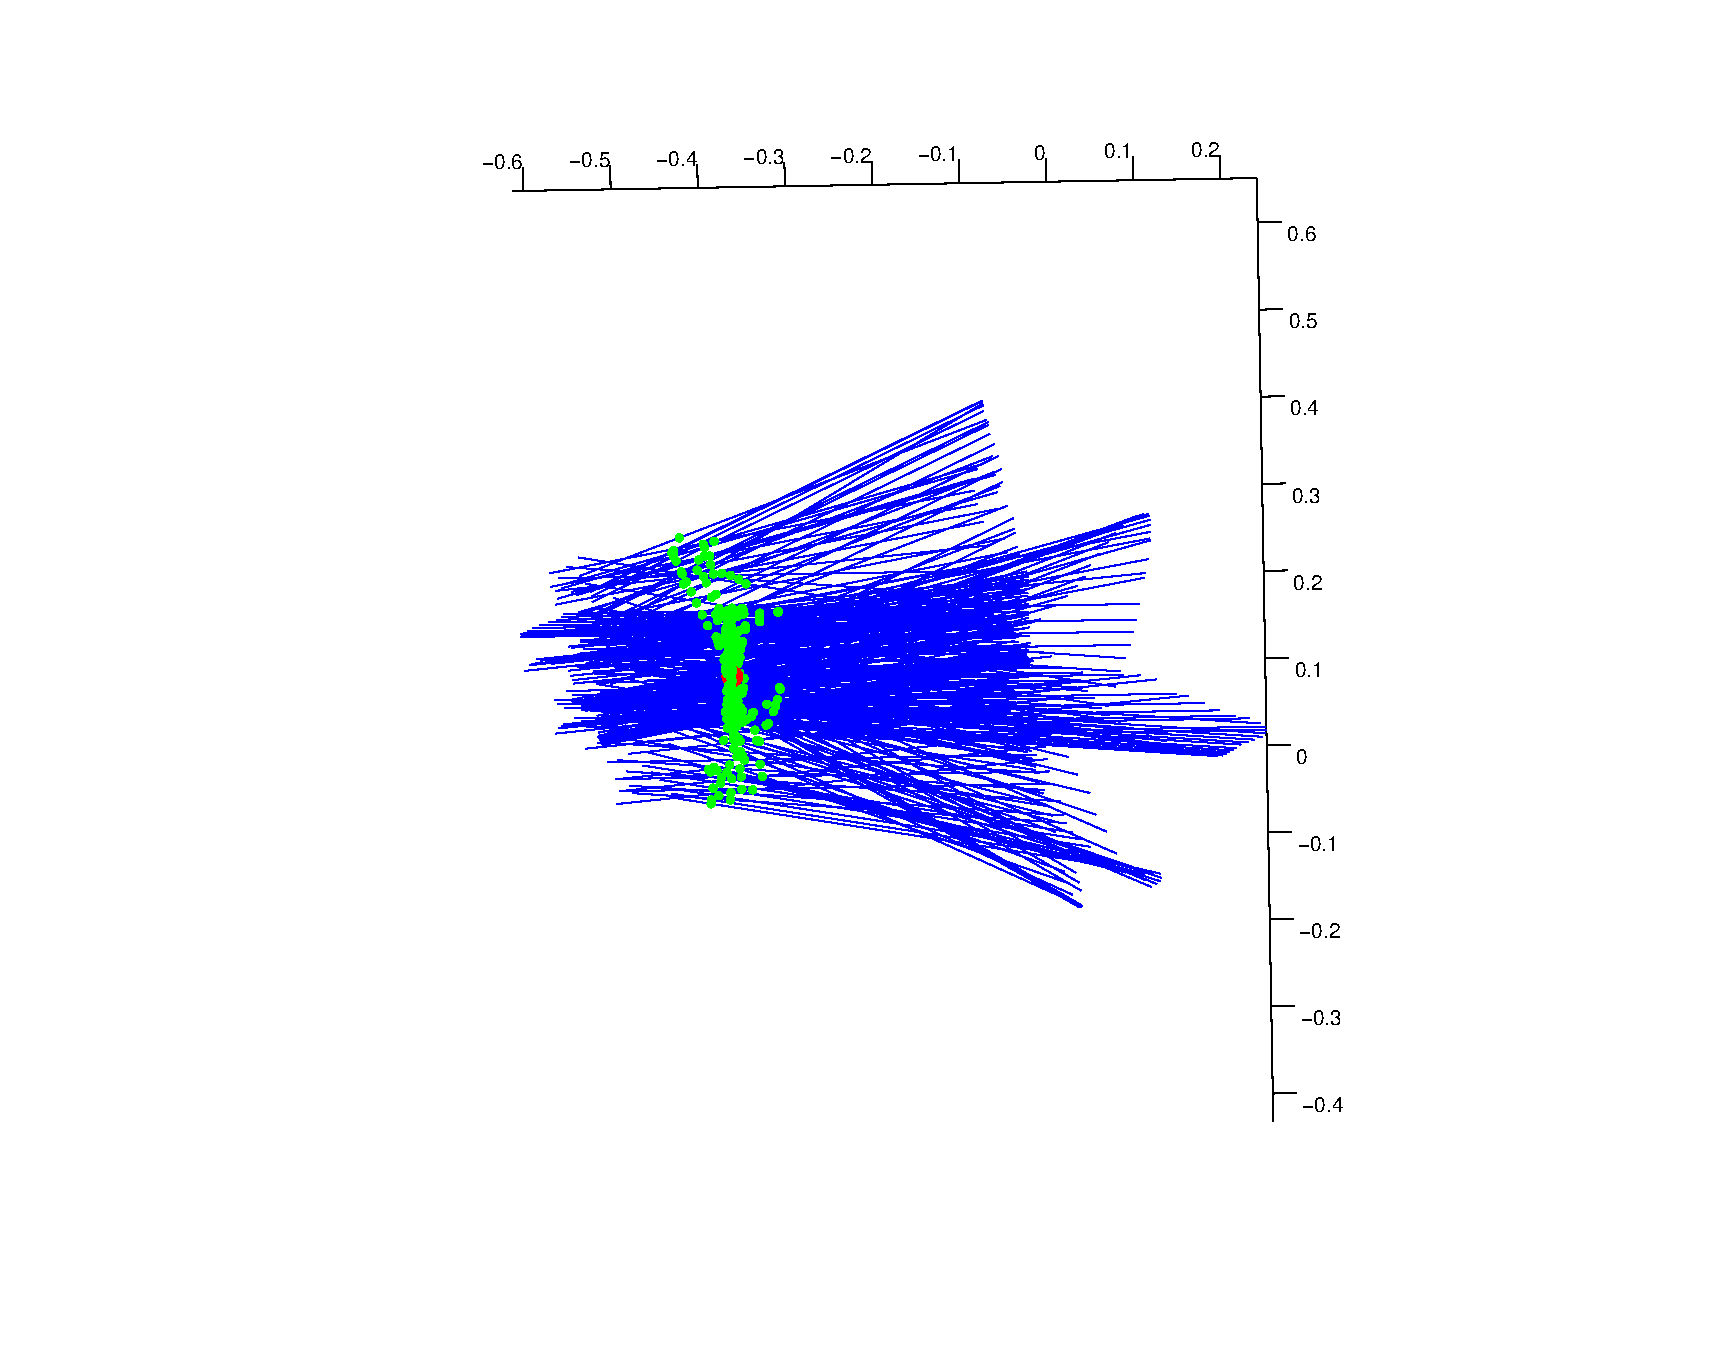
\includegraphics[width=1.1\linewidth]{./img/loc_calib_gauss.eps}
	\end{subfigure}
	\hfill
	\begin{subfigure}[b]{0.49\textwidth}
		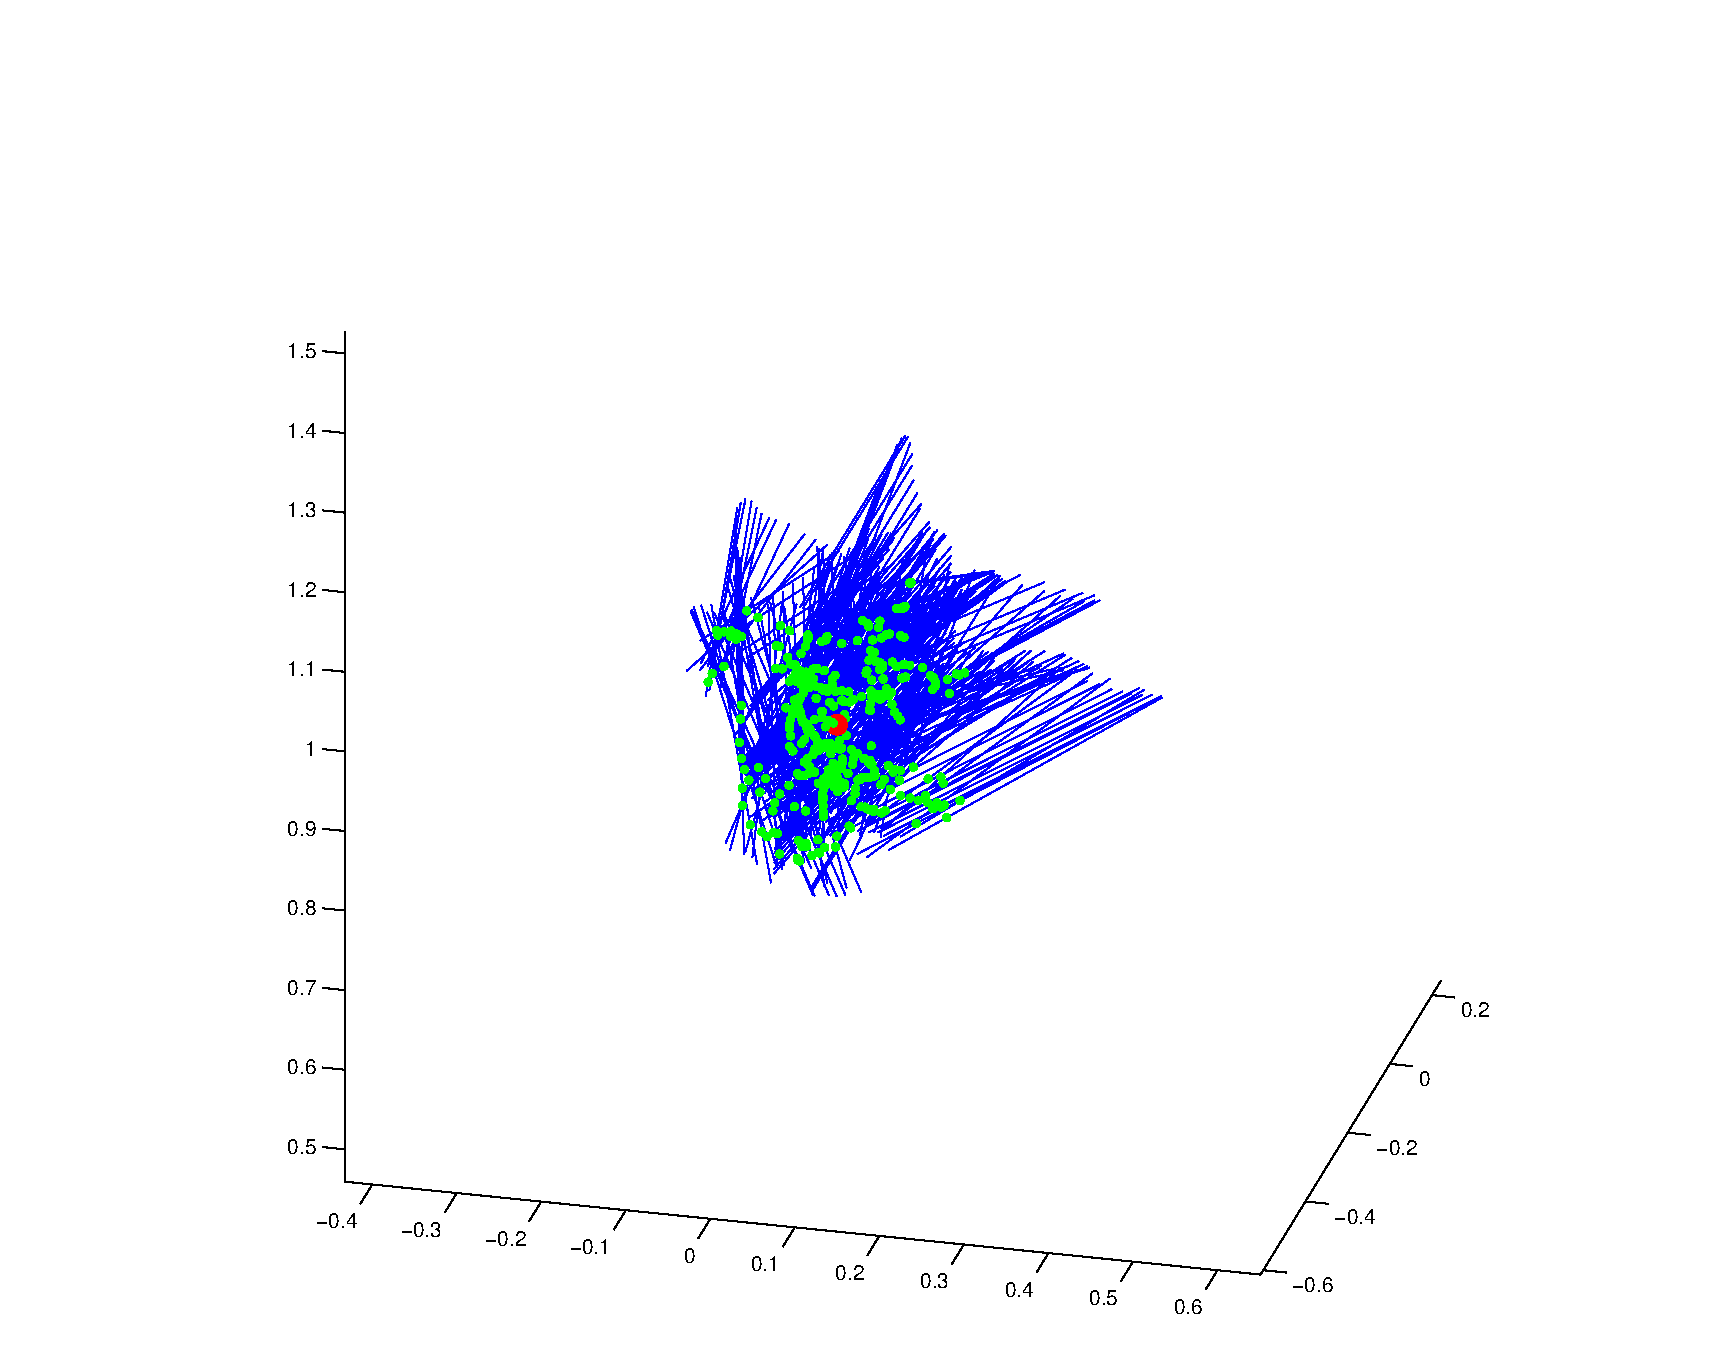
\includegraphics[width=1.1\linewidth]{./img/loc_calib_gauss_cross.eps}
	\end{subfigure}
	\caption{The Gaussian ellipsoid formed by finding the point of minimal sum of squared distances from all gaze lines.  Shown in red is the calculated point, shown in green are the closest point on each gaze line, shown in blue are the gaze lines.  In the left figure, the person doing the object location calibration is standing on the right, looking to the left.  The figure on the right shows the same plot rotated so the spread of the ellipsoid is seen more clearly.}
	\label{fig:locCalibResults}
\end{figure}

After this calibration for the objects of interest, we use a simple heuristic when identifying the object under gaze.  If gaze direction lies within x variance away from an object location mean, then this object is considered to be gazed at (x is a sensitivity parameter chosen manually).  If the gaze lies in two or more objects' vicinities, the object whose distance from gaze normalized by variance is less is chosen as the object under gaze.  If no objects are close to the gaze direction, the person is considered not looking at any object, i.e. idling.